\documentclass[hyperref=colorlinks]{beamer}
\mode<presentation>
\usetheme{iclpt}
\setbeamertemplate{navigation symbols}{}
\setbeamertemplate{headline}{
\begin{beamercolorbox}[leftskip=.2cm,rightskip=.2cm,topskip=.2cm,ht=1.1cm,dp=0.1cm,wd=\textwidth]{institute in head/foot}
  
\includegraphics[height=1cm]{icl.pdf}
  \hfill
  
\includegraphics[height=1cm]{../Pics/CMS-Color.pdf}
\end{beamercolorbox}
}
\setbeamertemplate{footline}{
\begin{beamercolorbox}[ht=.55cm,dp=0.4cm,wd=\textwidth,leftskip=.3cm]{author in head/foot}%
  \begin{minipage}[c]{5cm}%
    \usebeamerfont{author in head/foot}
    \insertshortauthor 
    \insertshorttitle
    \end{minipage}\hfill%
  \insertframenumber{} / \pageref{lastframe}
  \hfill
  \begin{minipage}{6cm}
    \hfill
  \end{minipage}
\end{beamercolorbox}%
}

\usepackage{color}
\usepackage{tabularx,colortbl}
\usepackage{graphicx}
\usepackage{pdfpages}
\usepackage{feynmp}
\DeclareGraphicsRule{*}{mps}{*}{}

\title{\vspace{-0.2cm} VBF Higgs to Invisible Update}
\subtitle{HIG-14-038, AN-14-243\vspace{-0.7cm}}
\author[]{}%\underline{P. Dunne}} % A.M. Magnan and A. Nikitenko Joao Pela with \\ R. Aggleton, J. Brooke: Bristol \\ C.Asawangtrakuldee, Q.Li: Peking \\ P. Srimanobhas: Chulalongkorn \\ S. Kumar, K. Mazumdar: Mumbai}
\titlegraphic{
  \vspace{-0.7cm}
  %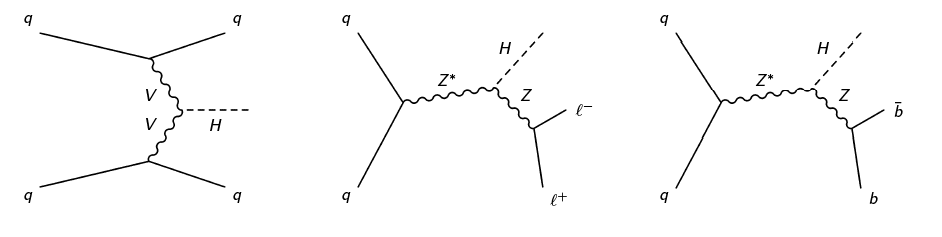
\includegraphics[width=\textwidth]{TalkPics/invcomb021213/feyndiags}
  %% \begin{fmfgraph*}(100,70)
  %%         \fmfleft{i1,i2}
  %%         \fmfright{o1,o2,o3}
  %%         \fmf{fermion}{i1,v1,o1}
  %%         \fmf{fermion}{i2,v2,o3}
  %%         \fmf{phantom,tension=4/5}{v1,v2}
  %%         \fmffreeze
  %%         \fmf{photon,label=$W,,Z$}{v1,v3}
  %%         \fmf{photon,label=$W,,Z$}{v2,v3}
  %%         \fmf{dashes}{v3,o2}
  %%         \fmflabel{$q$}{i1}
  %%         \fmflabel{$q$}{i2}
  %%         \fmflabel{$q$}{o1}
  %%         \fmflabel{$q$}{o3}
  %%         \fmflabel{$H$}{o2}
  %%       \end{fmfgraph*}
}
\date{}
\begin{document}
\begin{fmffile}{higgsexoupdatefeyndiags}

%TITLE PAGE
\section{Title}
\begin{frame}
  \titlepage
  
\end{frame}

\begin{frame}
  \frametitle{Yields}
  \centering
  \begin{tabular}{lc}
\hline \hline
Process & Event yields \\
\hline
$Z\rightarrow\nu\nu$&$158.1 \pm 37.3 \pm 21.2$\\
$W\rightarrow\mu\nu$&$102.5 \pm 6.2 \pm 11.7$\\
$W\rightarrow e\nu$&$57.9 \pm 7.4 \pm 7.7$\\
$W\rightarrow\tau\nu$&$94.6 \pm 13.1 \pm 23.8$\\
top&$5.5 \pm  1.8$\\
VV&$3.9 \pm 0.7$\\
QCD multijet &$17\pm 14$\\
\hline
Total Background &$439.4 \pm 40.7 \pm 43.5 $\\
\hline
Signal(VBF) &$273.1 \pm 31.2 $\\
Signal(ggH) &$23.1 \pm 15.9 $\\
\hline
Observed data & 508 \\
\hline \hline
  \end{tabular}
\end{frame}

\begin{frame}
  \frametitle{QCD}
  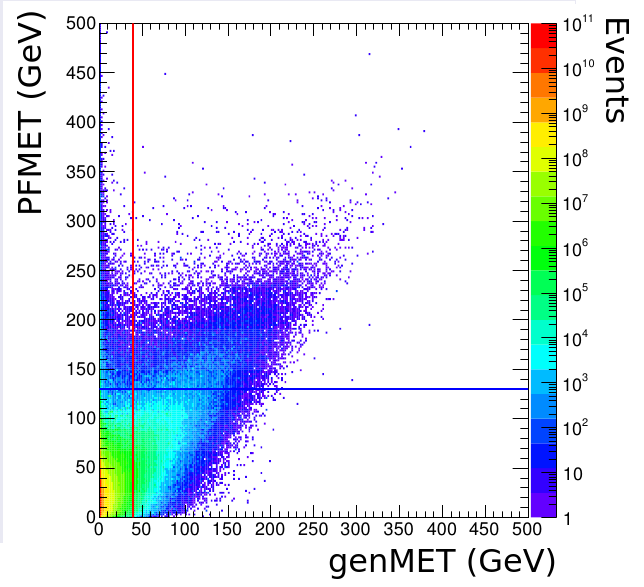
\includegraphics[width=.5\textwidth,height=.7\textheight]{TalkPics/studentseminar130415/Joao_140209_p11.png}
  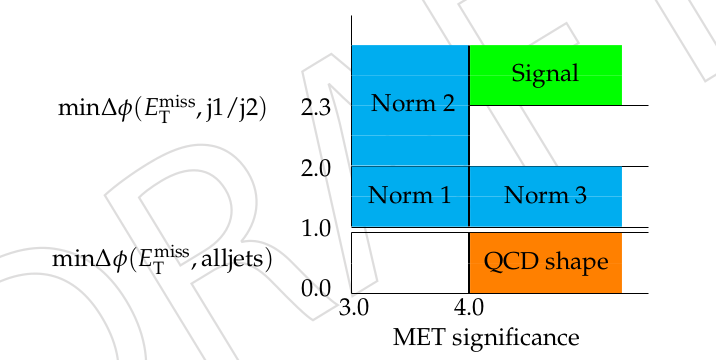
\includegraphics[width=.5\textwidth,height=.7\textheight]{TalkPics/studentseminar130415/schema.png}
\end{frame}

\begin{frame}
  \frametitle{QCD}
  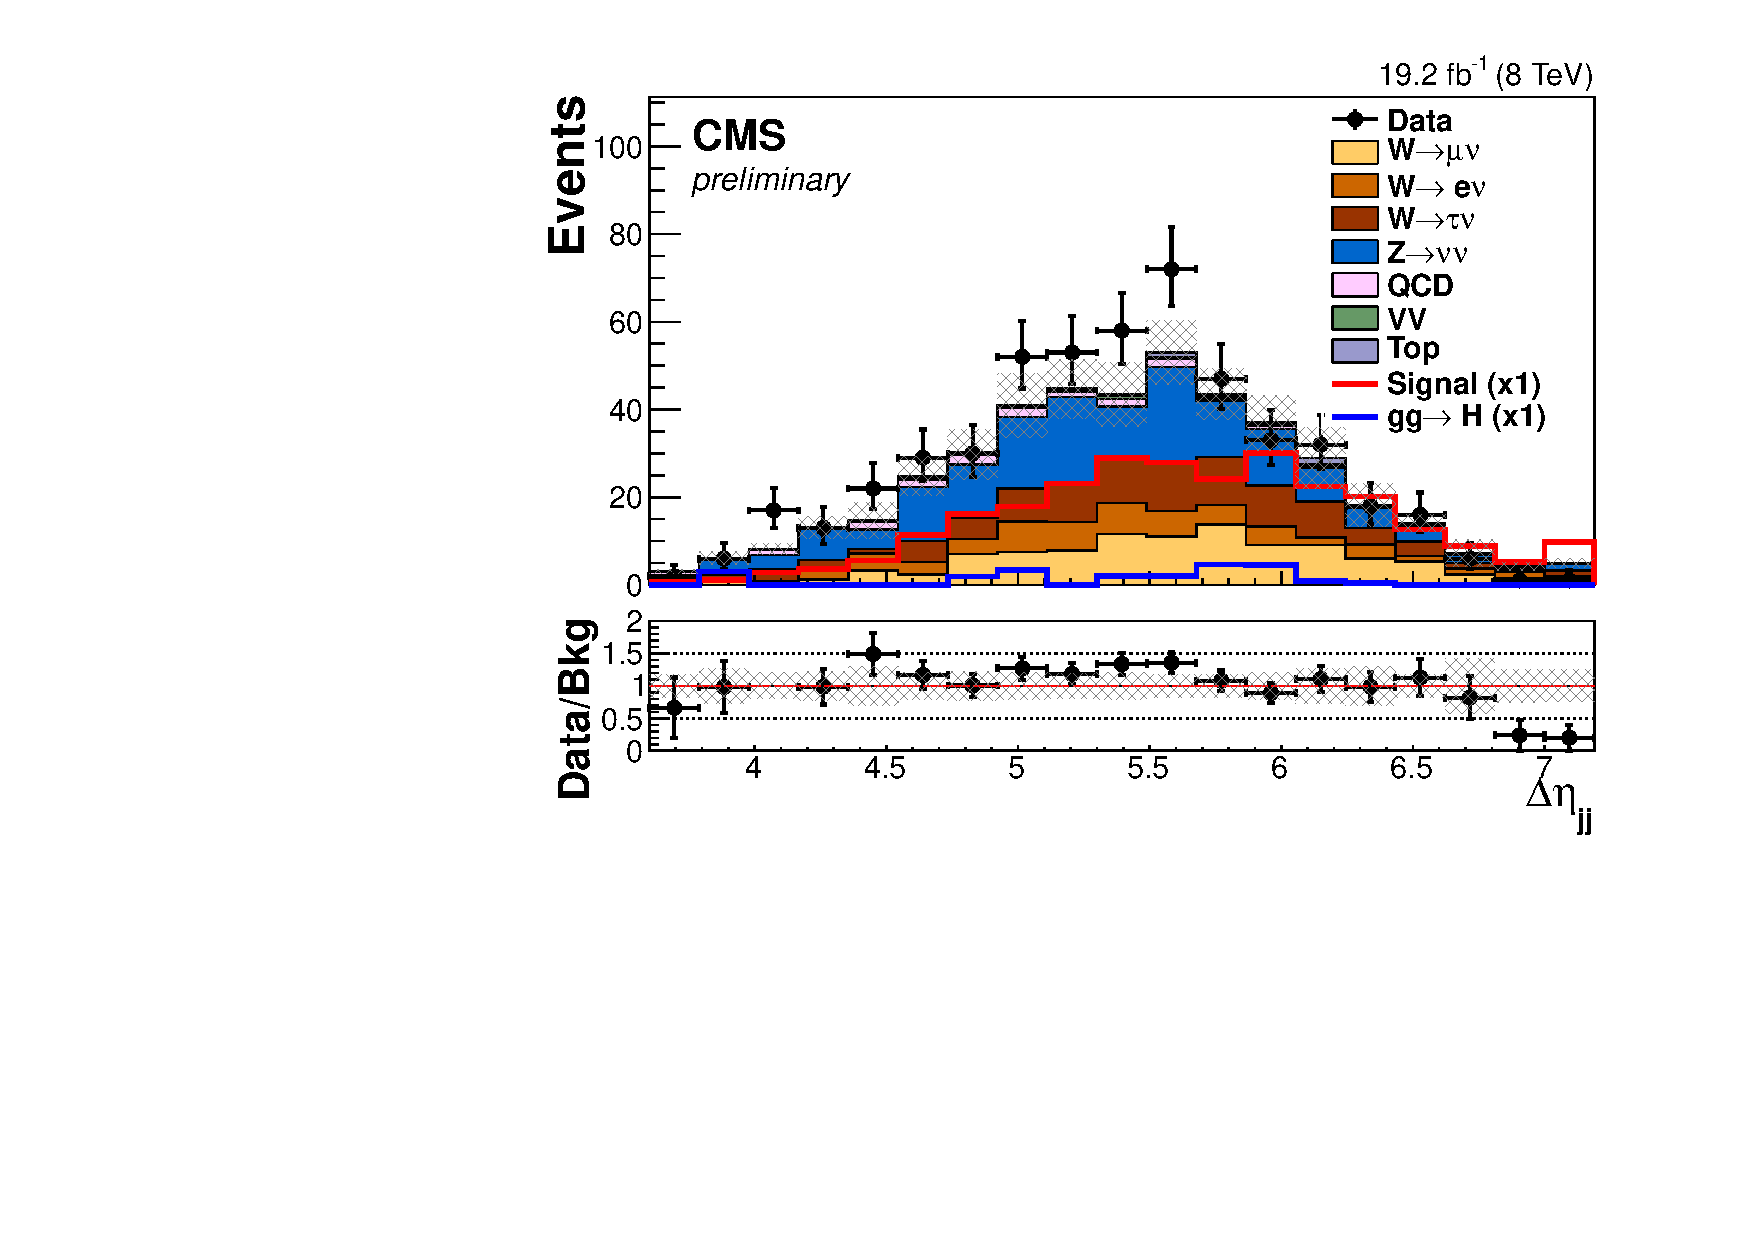
\includegraphics[width=.5\textwidth,height=.7\textheight]{TalkPics/studentseminar130415/nunu_dijet_deta.pdf}
  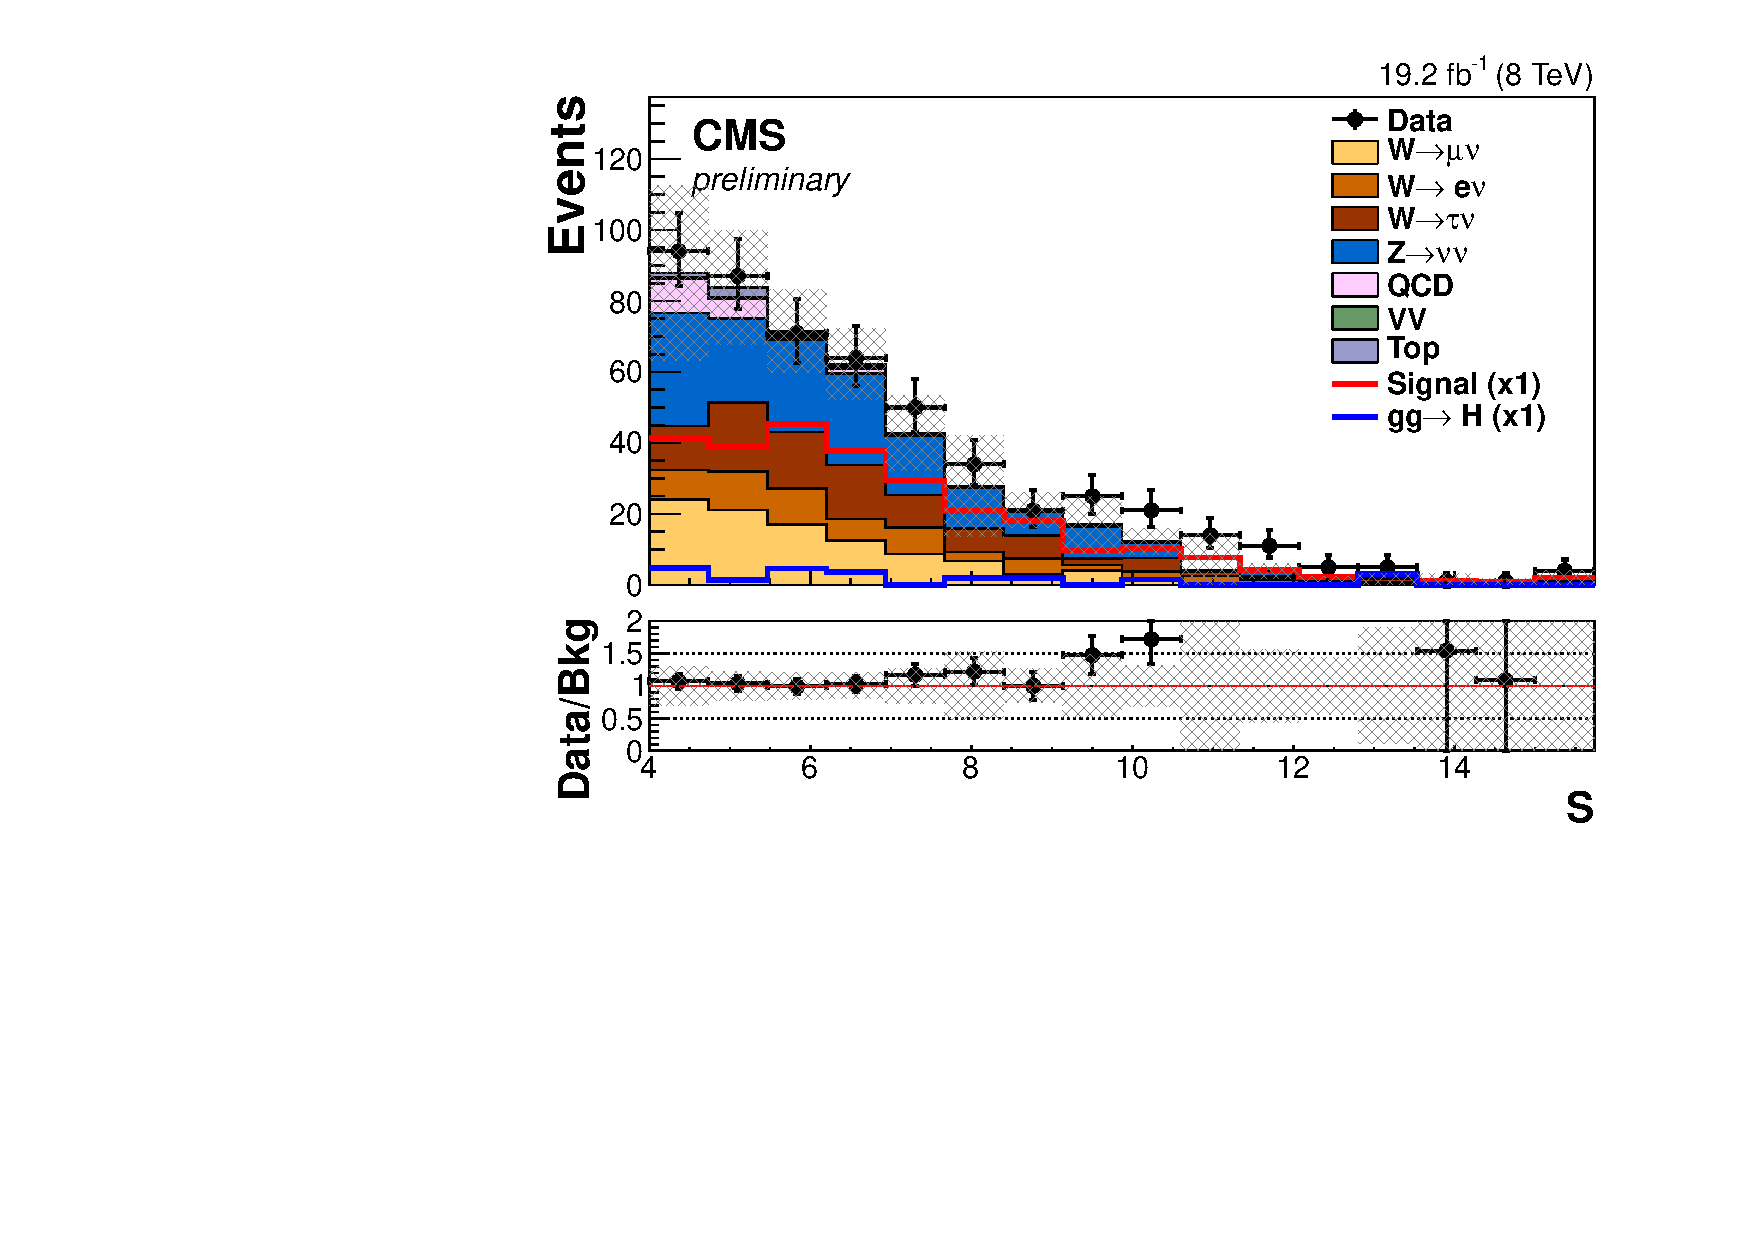
\includegraphics[width=.5\textwidth,height=.7\textheight]{TalkPics/studentseminar130415/nunu_metnomu_significance.pdf}
\end{frame}

\begin{frame}
  %NEVENTS INSIDE VS OUTSIDE, GOOD AGREEMENT INSIDE ACCEPTANCE, BAD OUTSIDE
  \frametitle{Inside/outside acceptance check}
  \begin{block}{}
    \scriptsize
    \begin{itemize}
    \item Check MC yield in signal region from  $W\rightarrow e/\mu\nu$
    \item[-] i.e. we veto any reconstructed leptons
    \item Split into events with gen lepton inside acceptance ($|\eta|<2.1$) and outside acceptance ($|\eta|>2.4$)
    \end{itemize}
    \begin{center}
      \begin{tabular}{|l|c|c|}
        \hline
        Process & Inside acceptance & Outside acceptance \\
        \hline
        $W\rightarrow e\nu$ & $73.7\pm 6.8$ &  $30.2\pm 4.9$ \\
        \hline
        $W\rightarrow \mu\nu$ & $61.5\pm 6.8$ & $74.4\pm 7.3$ \\
        \hline
      \end{tabular}
      \end{center}
      \begin{itemize}
      \item Inside acceptance:
      \item[-] Slightly more e$\nu$ events
      \item[-] Might be from efficiency 
      \item Outside acceptance results odd
      \end{itemize}
  \end{block}
\end{frame}


\begin{frame}
  \frametitle{Shape checks inside acceptance}
  \vspace{-.3cm}
  \begin{center}
    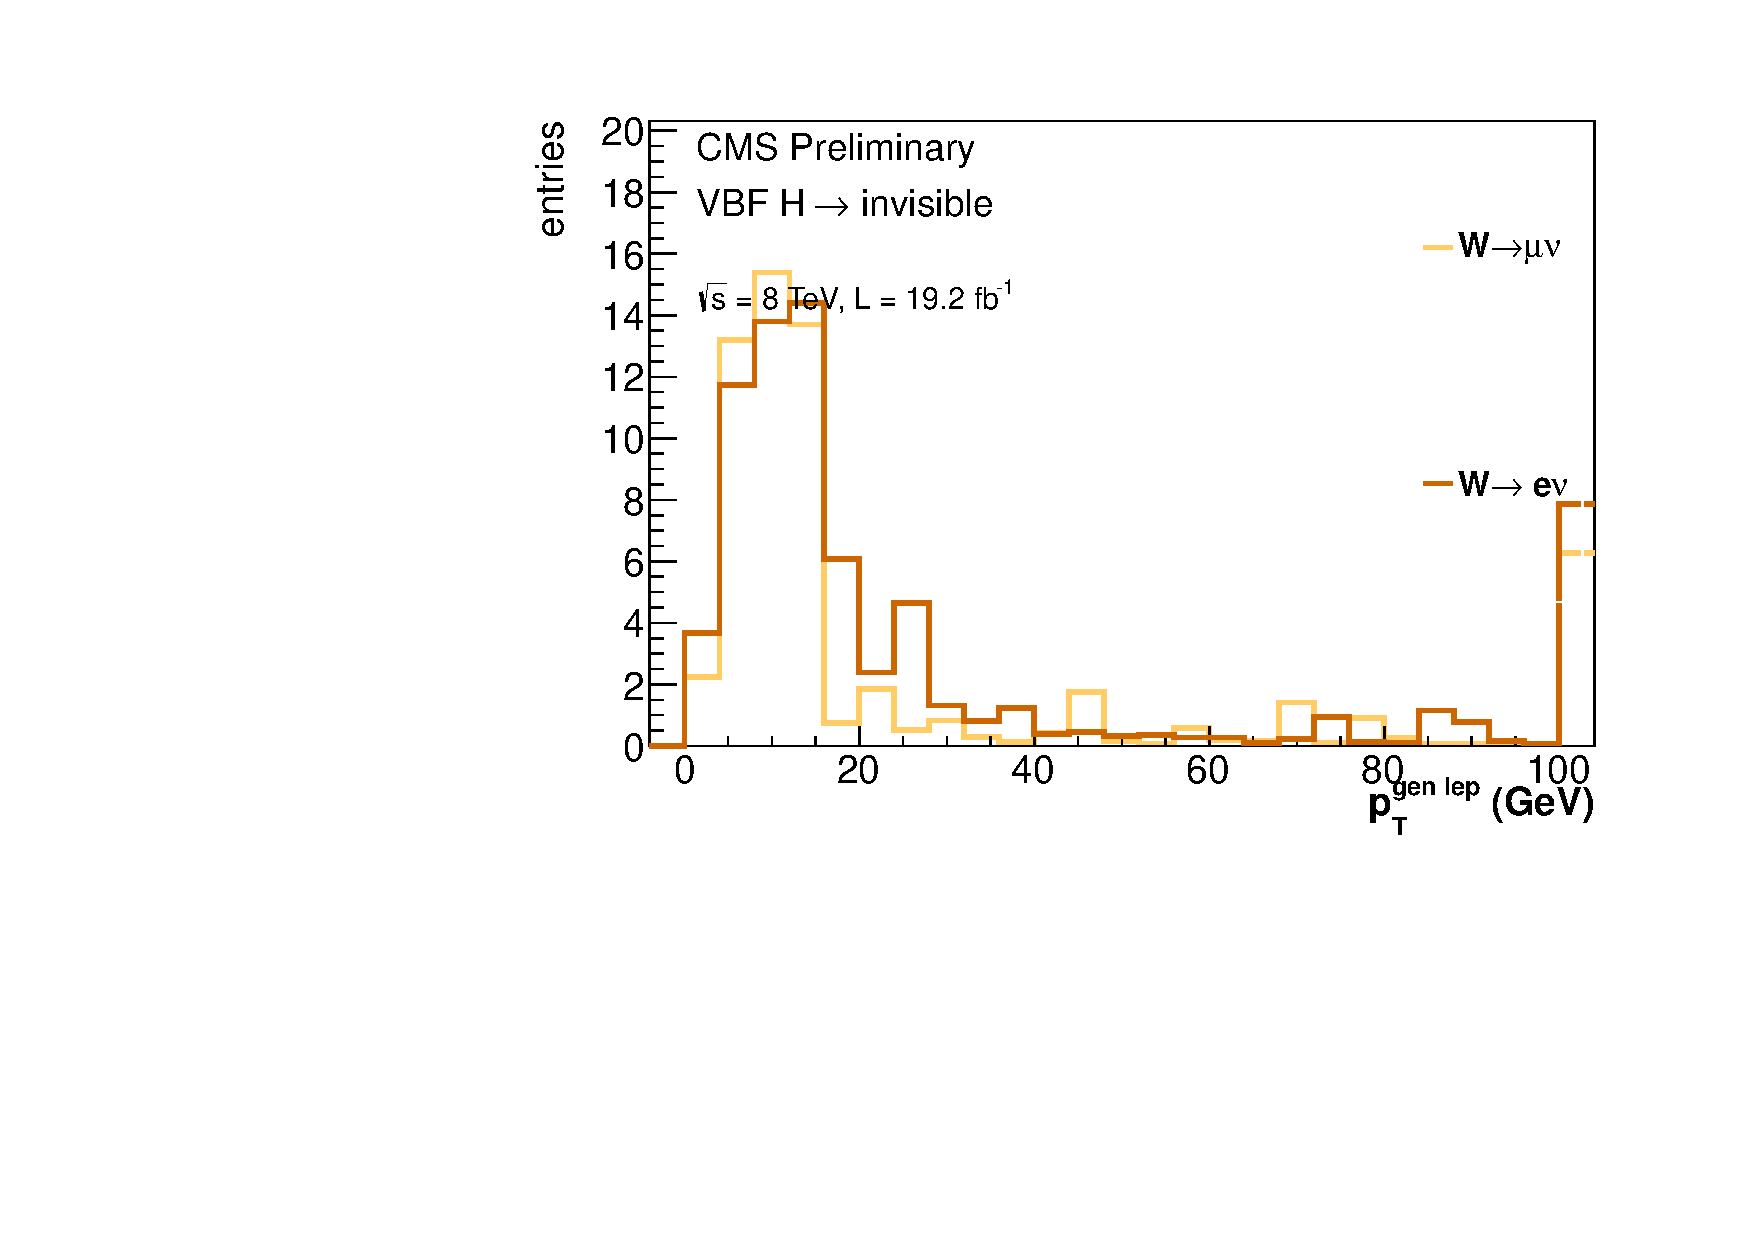
\includegraphics[width=.4\textwidth,clip=true,trim=0 0 0 30]{TalkPics/genlepstudy020315/insideacceptancetightdphi/nunu_genlep1_pt.pdf}
    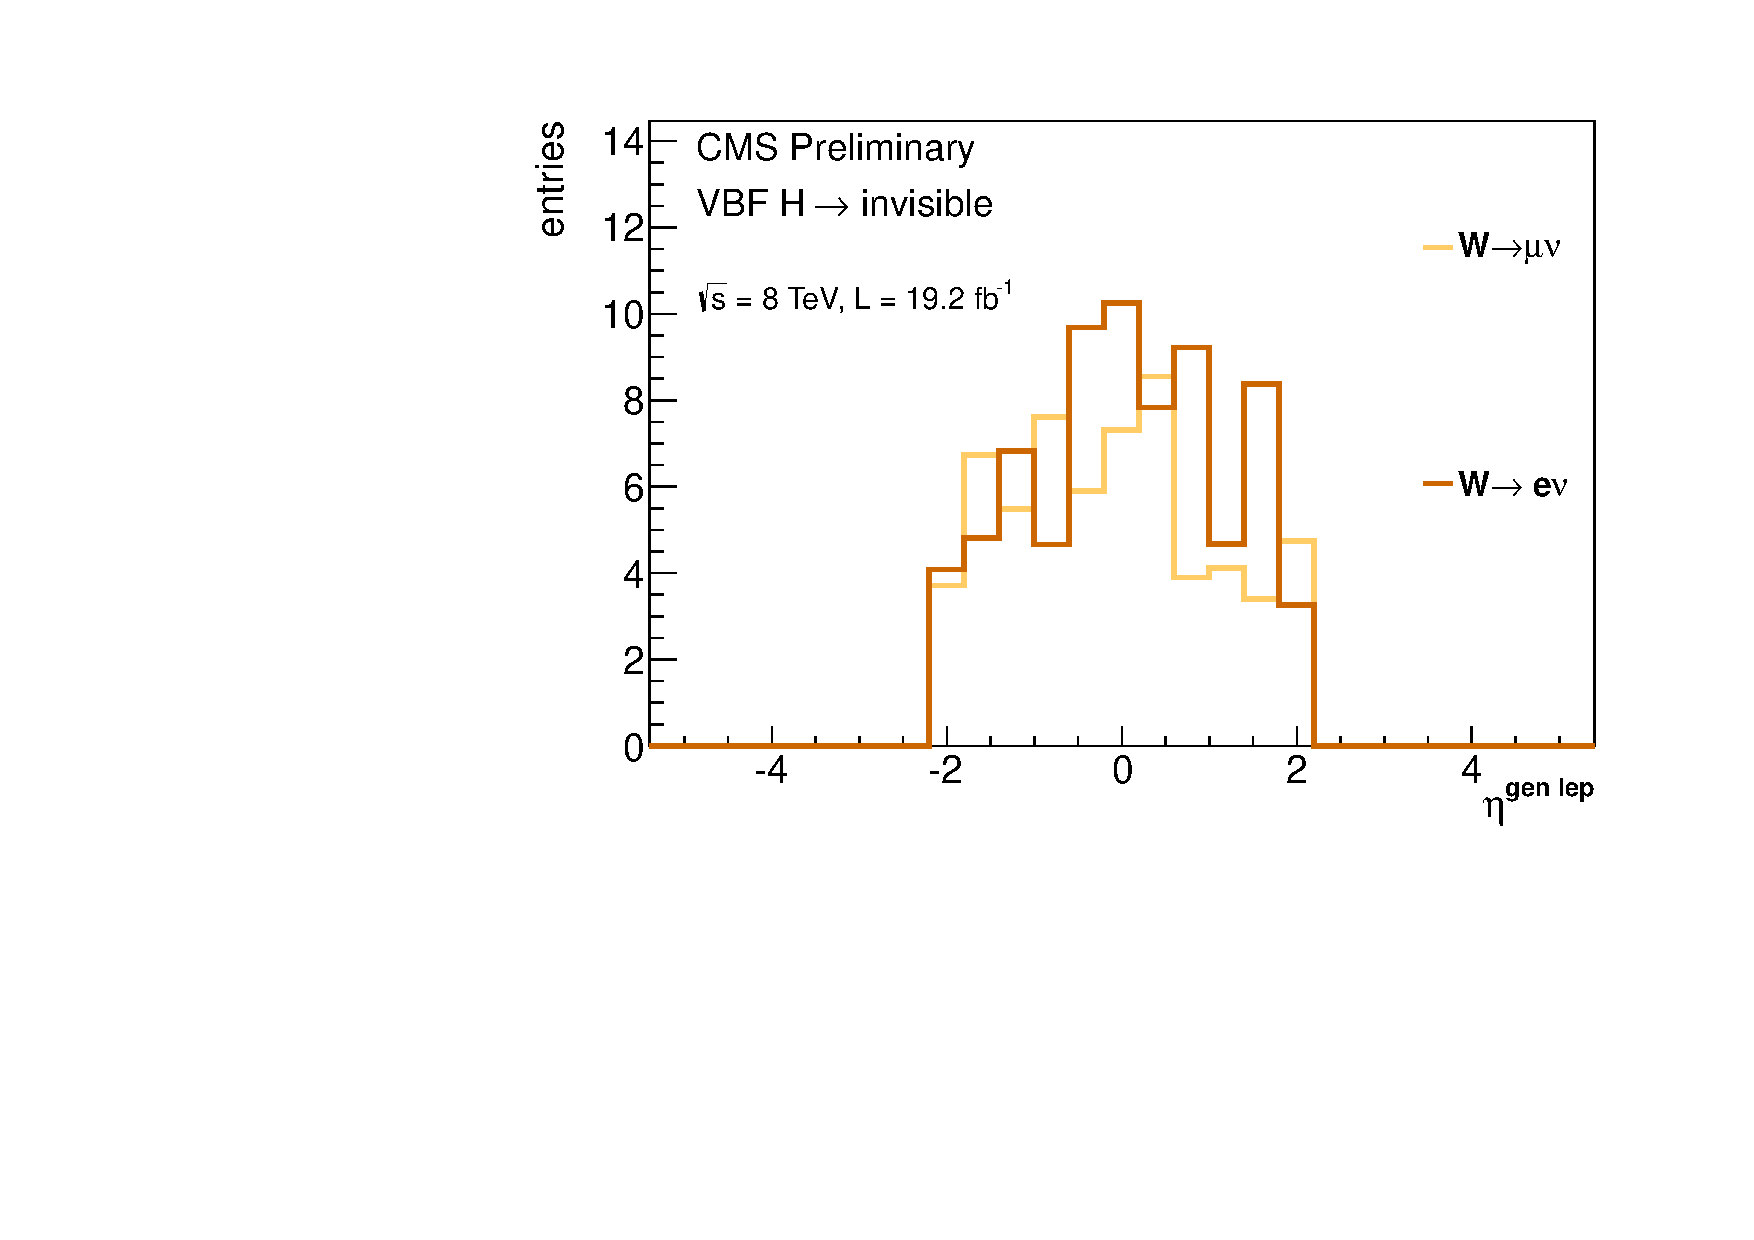
\includegraphics[width=.4\textwidth,clip=true,trim=0 0 0 30]{TalkPics/genlepstudy020315/insideacceptancetightdphi/nunu_genlep1_eta.pdf}

    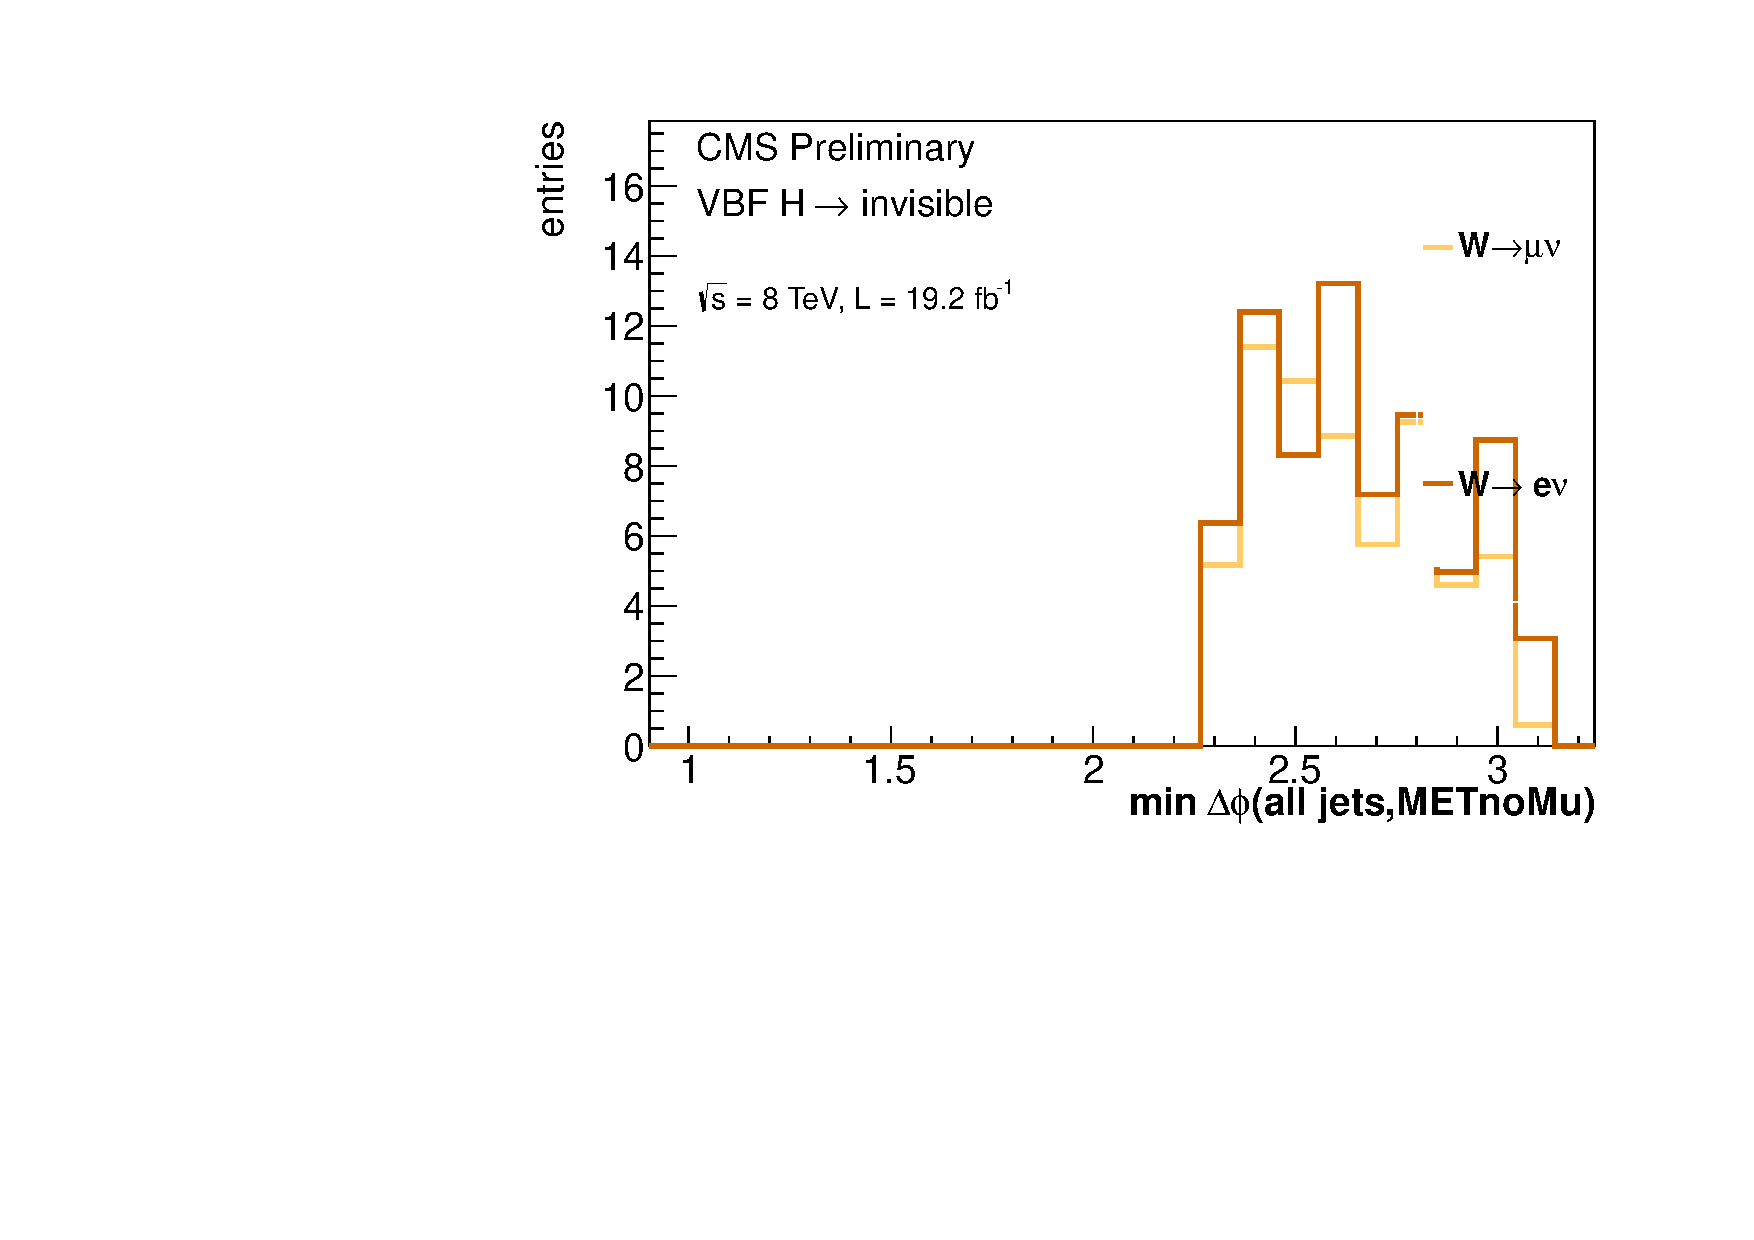
\includegraphics[width=.4\textwidth,clip=true,trim=0 0 0 30]{TalkPics/genlepstudy020315/insideacceptancetightdphi/nunu_alljetsmetnomu_mindphi.pdf}
    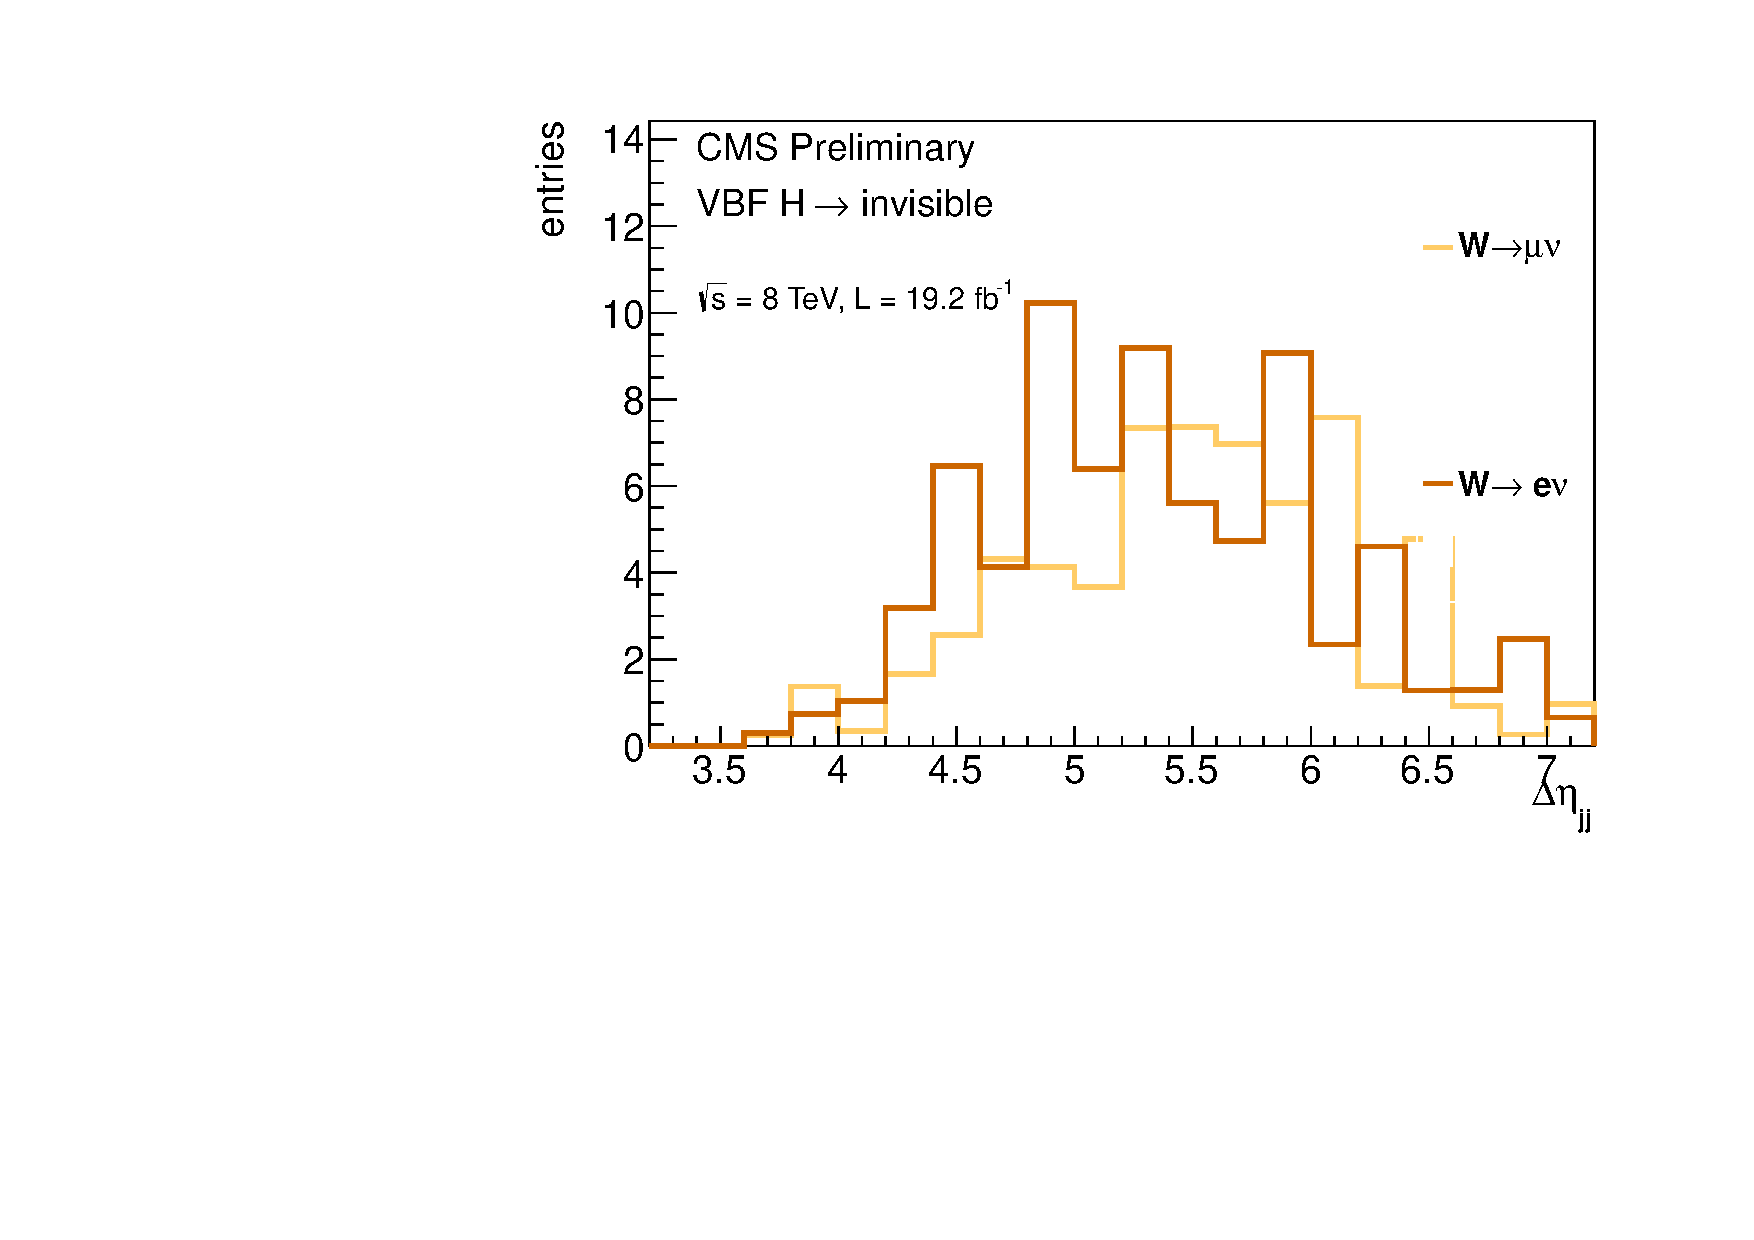
\includegraphics[width=.4\textwidth,clip=true,trim=0 0 0 30]{TalkPics/genlepstudy020315/insideacceptancetightdphi/nunu_dijet_deta.pdf}
    \end{center}
  %!!FIRST SHOW GOOD SHAPE AGREEMENT INSIDE, E MU EFF NOT SAME SO EXPECTED
\end{frame}

\begin{frame}
  %!!SHOW NJETS, MINDPHI, GENLEPPT AS EVIDENCE FOR ELE BECOMING JETS OUTSIDE ACCEPTANCE
  \frametitle{Outside acceptance}
    \begin{block}{}
    \scriptsize
    \begin{itemize}
    \item Outside acceptance $e\nu$ events have a lot more jets
    \item No $e\nu$ events with high pt gen leptons
    \end{itemize}
  \end{block}
  \begin{center}
    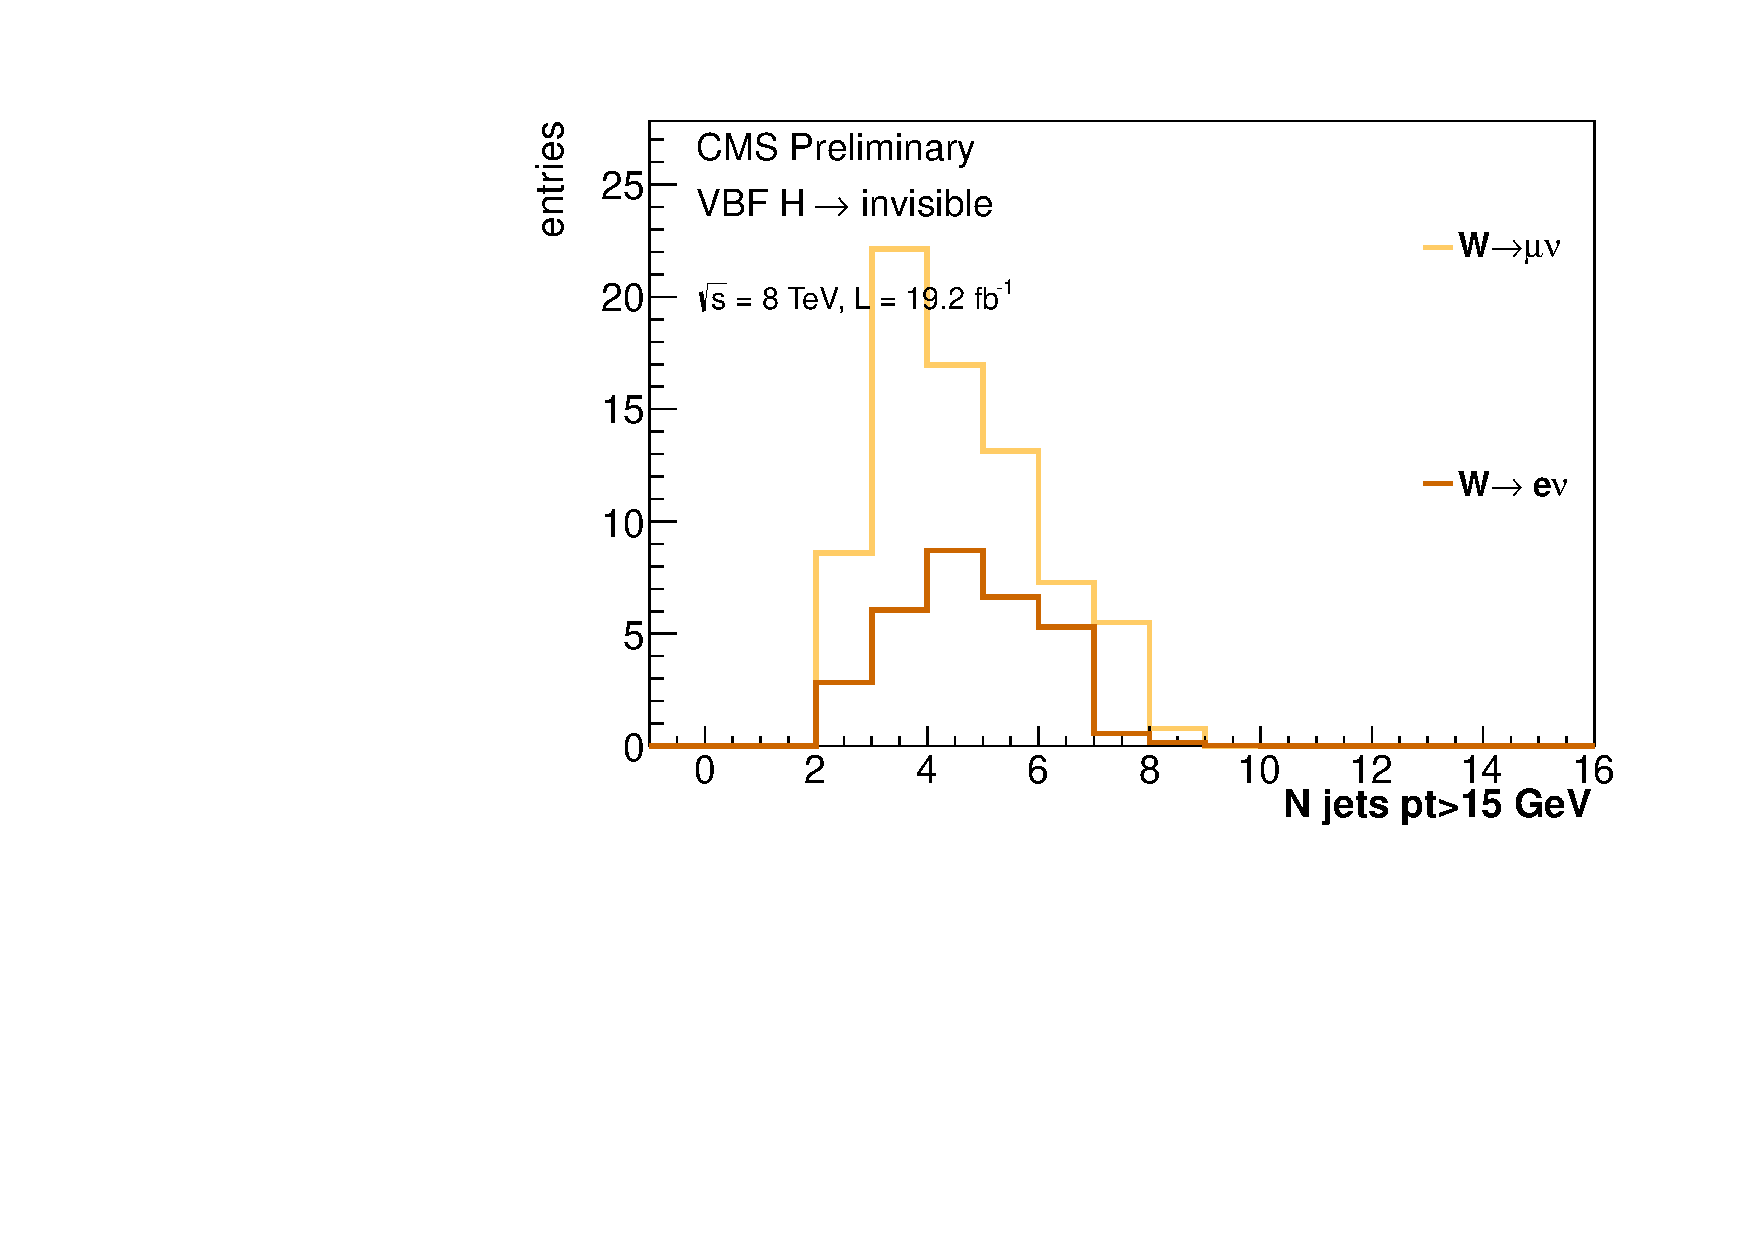
\includegraphics[width=.4\textwidth,height=.35\textheight,clip=true,trim=0 0 0 30]{TalkPics/genlepstudy020315/outsideacceptancetightdphi/nunu_n_jets_15.pdf}
    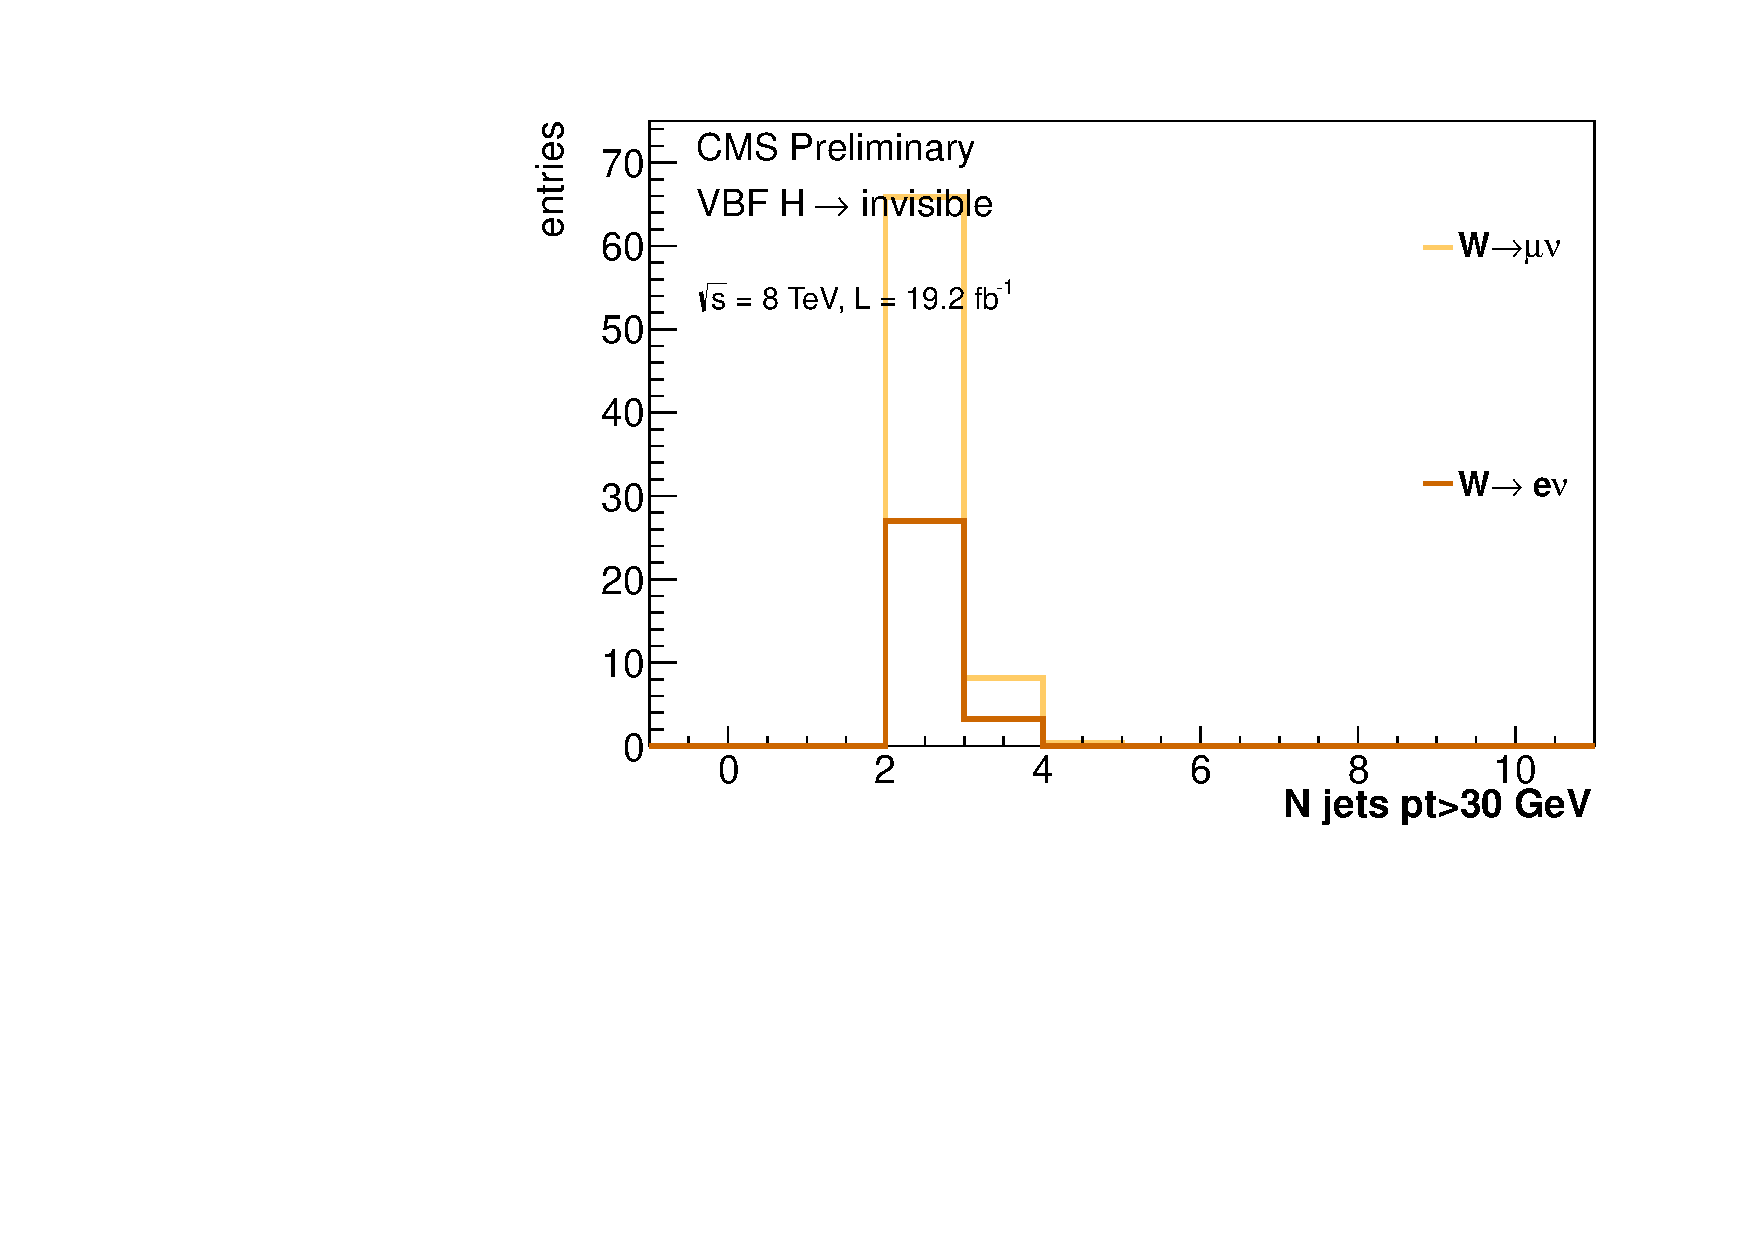
\includegraphics[width=.4\textwidth,height=.35\textheight,clip=true,trim=0 0 0 30]{TalkPics/genlepstudy020315/outsideacceptancetightdphi/nunu_n_jets_30.pdf}


    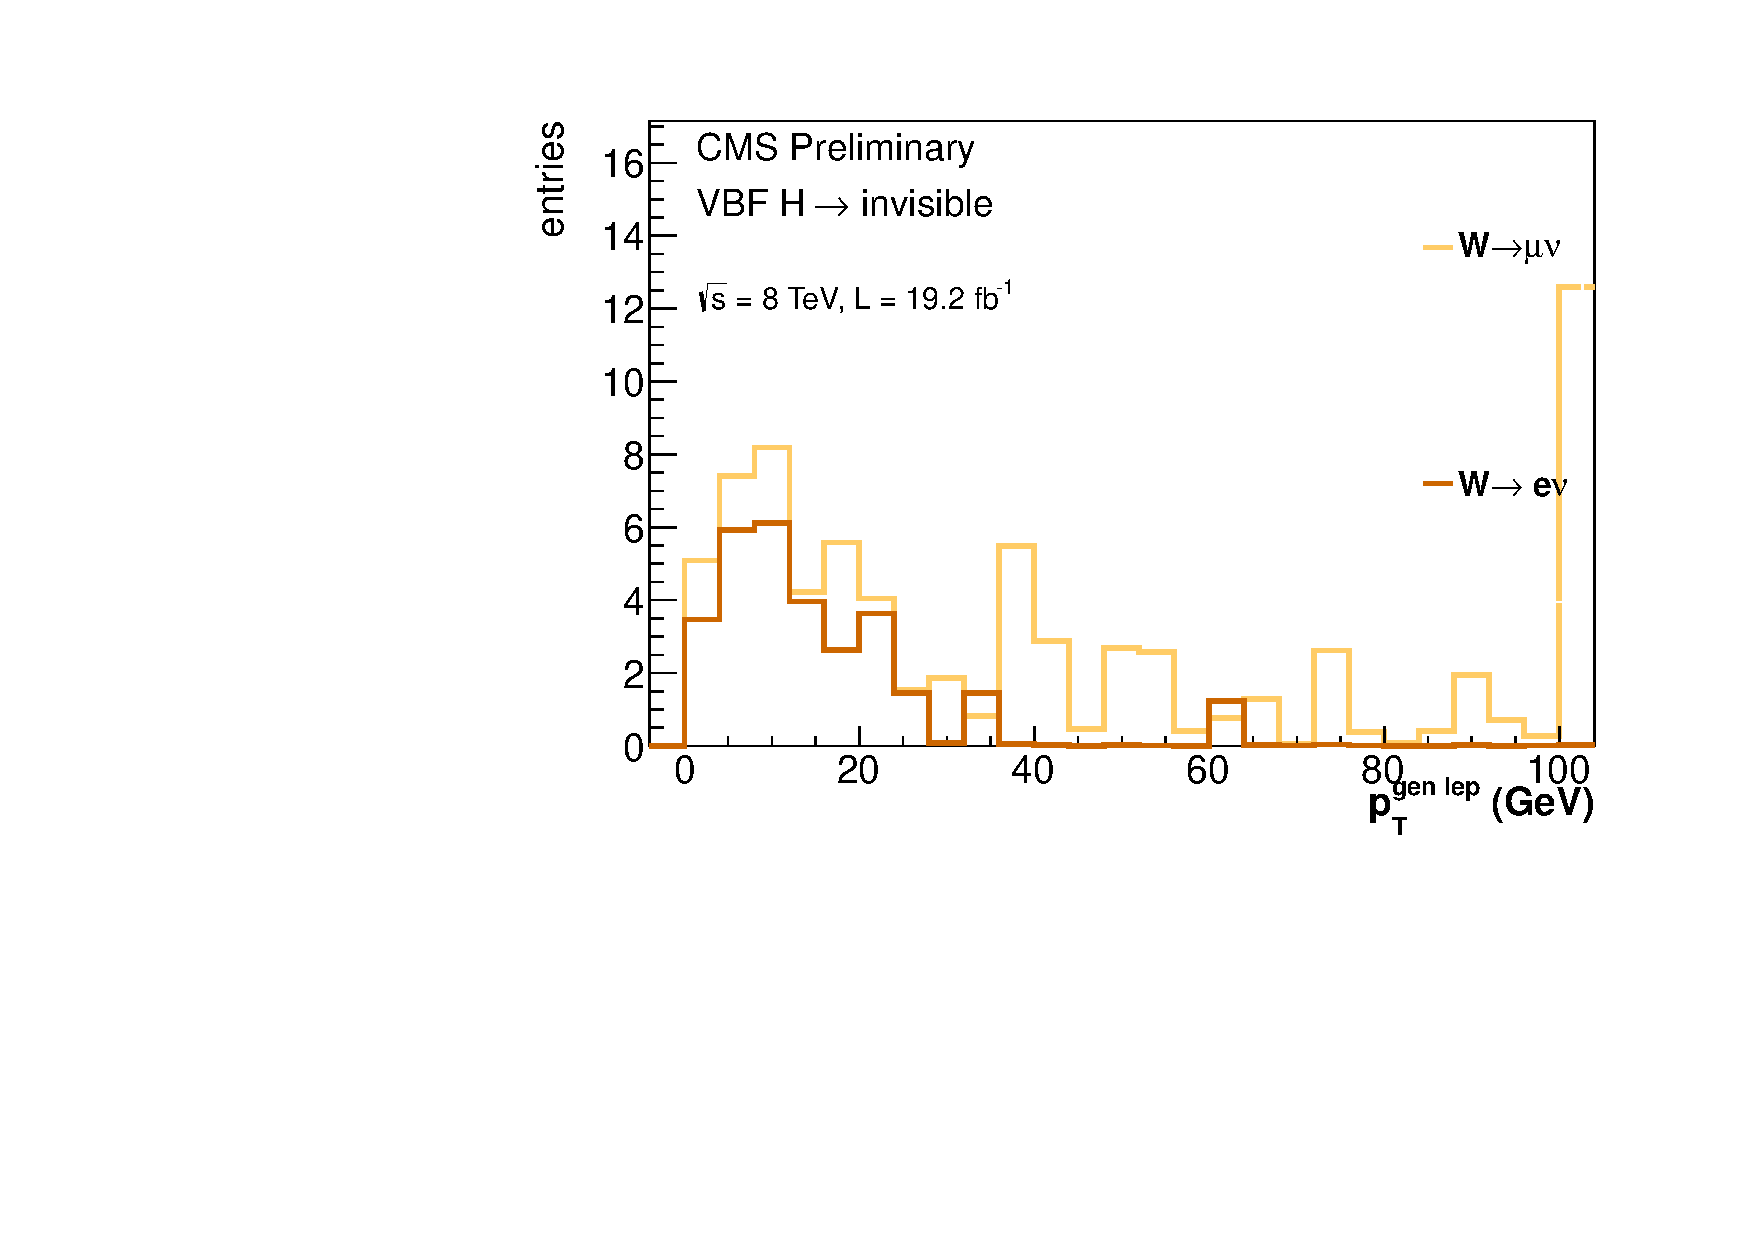
\includegraphics[width=.4\textwidth,height=.35\textheight,clip=true,trim=0 0 0 30]{TalkPics/genlepstudy020315/outsideacceptancetightdphi/nunu_genlep1_pt.pdf}
    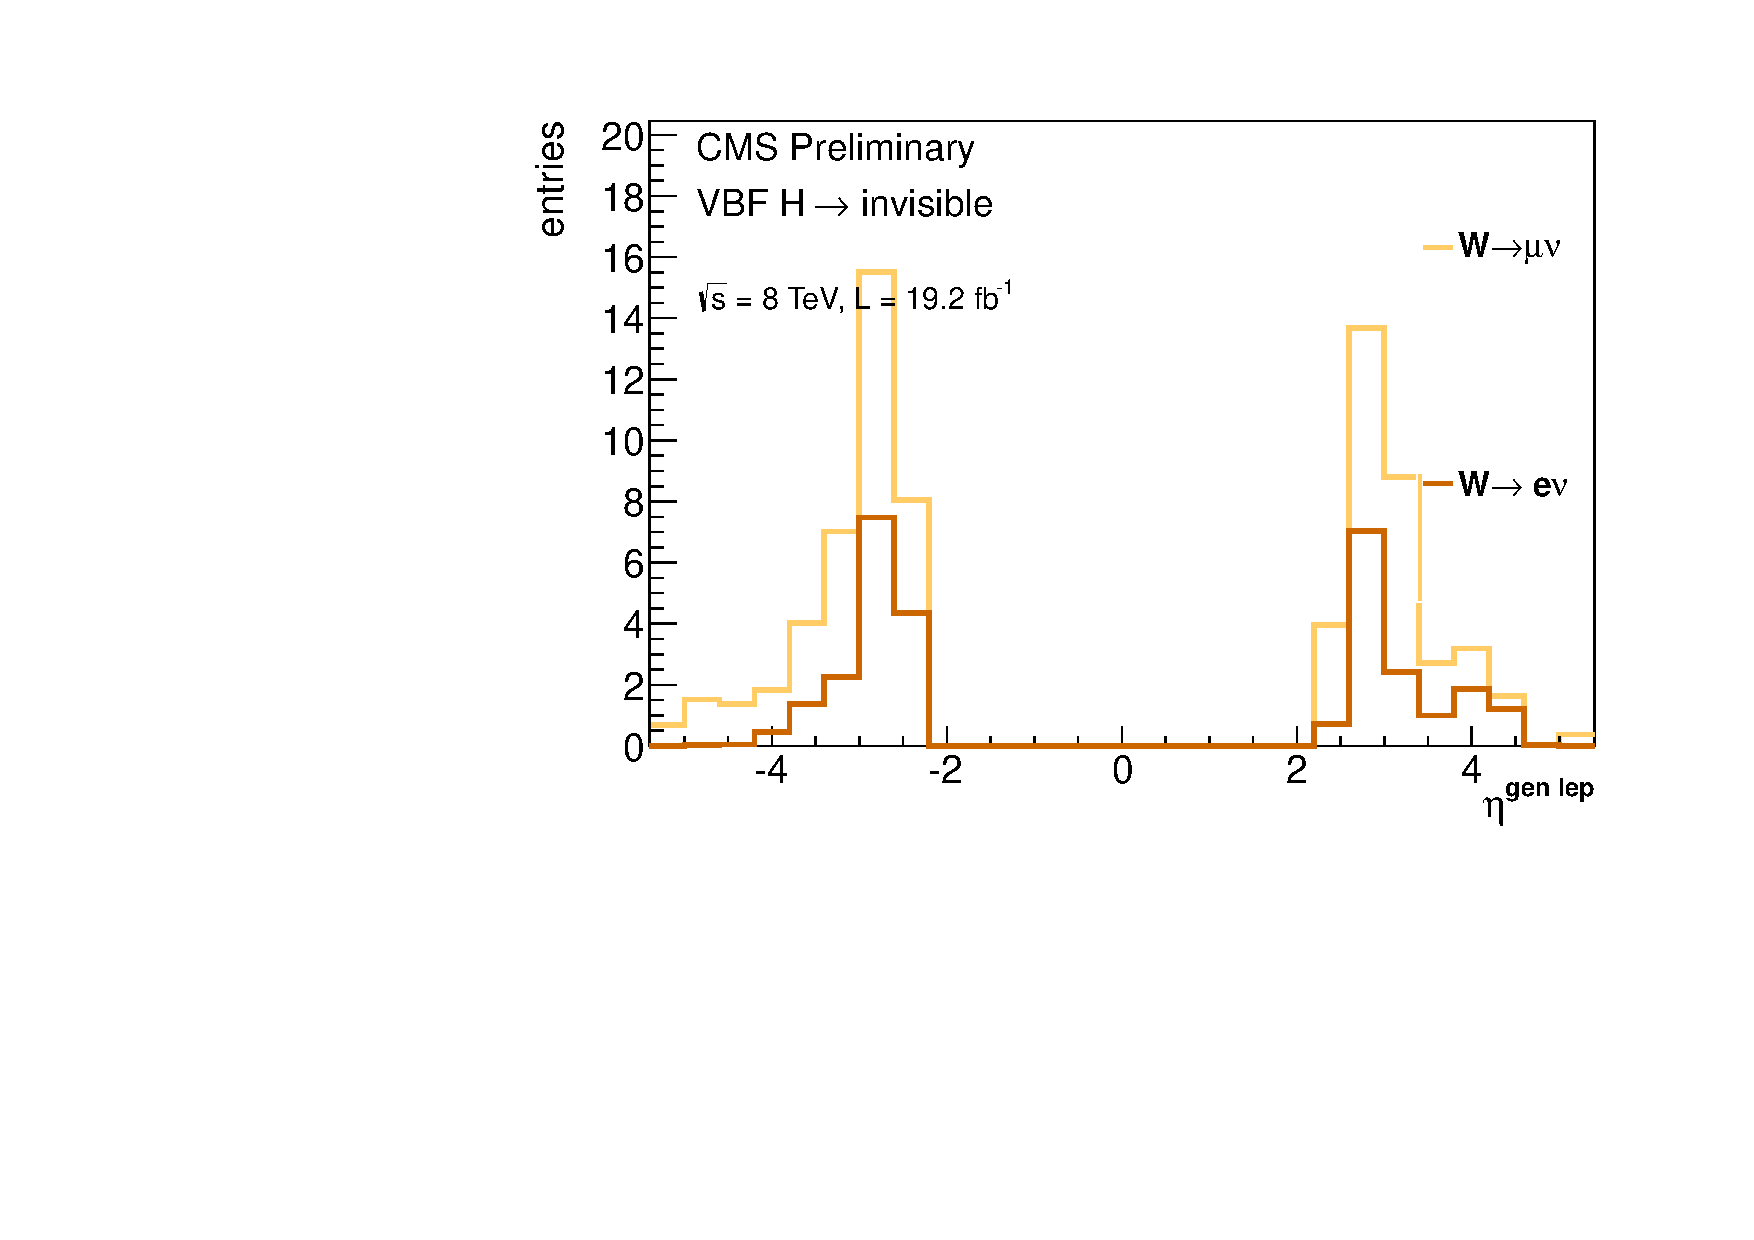
\includegraphics[width=.4\textwidth,height=.35\textheight,clip=true,trim=0 0 0 30]{TalkPics/genlepstudy020315/outsideacceptancetightdphi/nunu_genlep1_eta.pdf}
    \end{center}

\end{frame}

\begin{frame}
  %!!SHOW NJETS, MINDPHI, GENLEPPT AS EVIDENCE FOR ELE BECOMING JETS OUTSIDE ACCEPTANCE
  \frametitle{Outside acceptance}
    \begin{block}{}
    \scriptsize
    \begin{itemize}
    \item Seems outside acceptance electrons are more likely to be reconstructed as jets than muons
    \item Loosen jetmetdphi cut to 1
    \end{itemize}
  \end{block}
  \begin{center}
    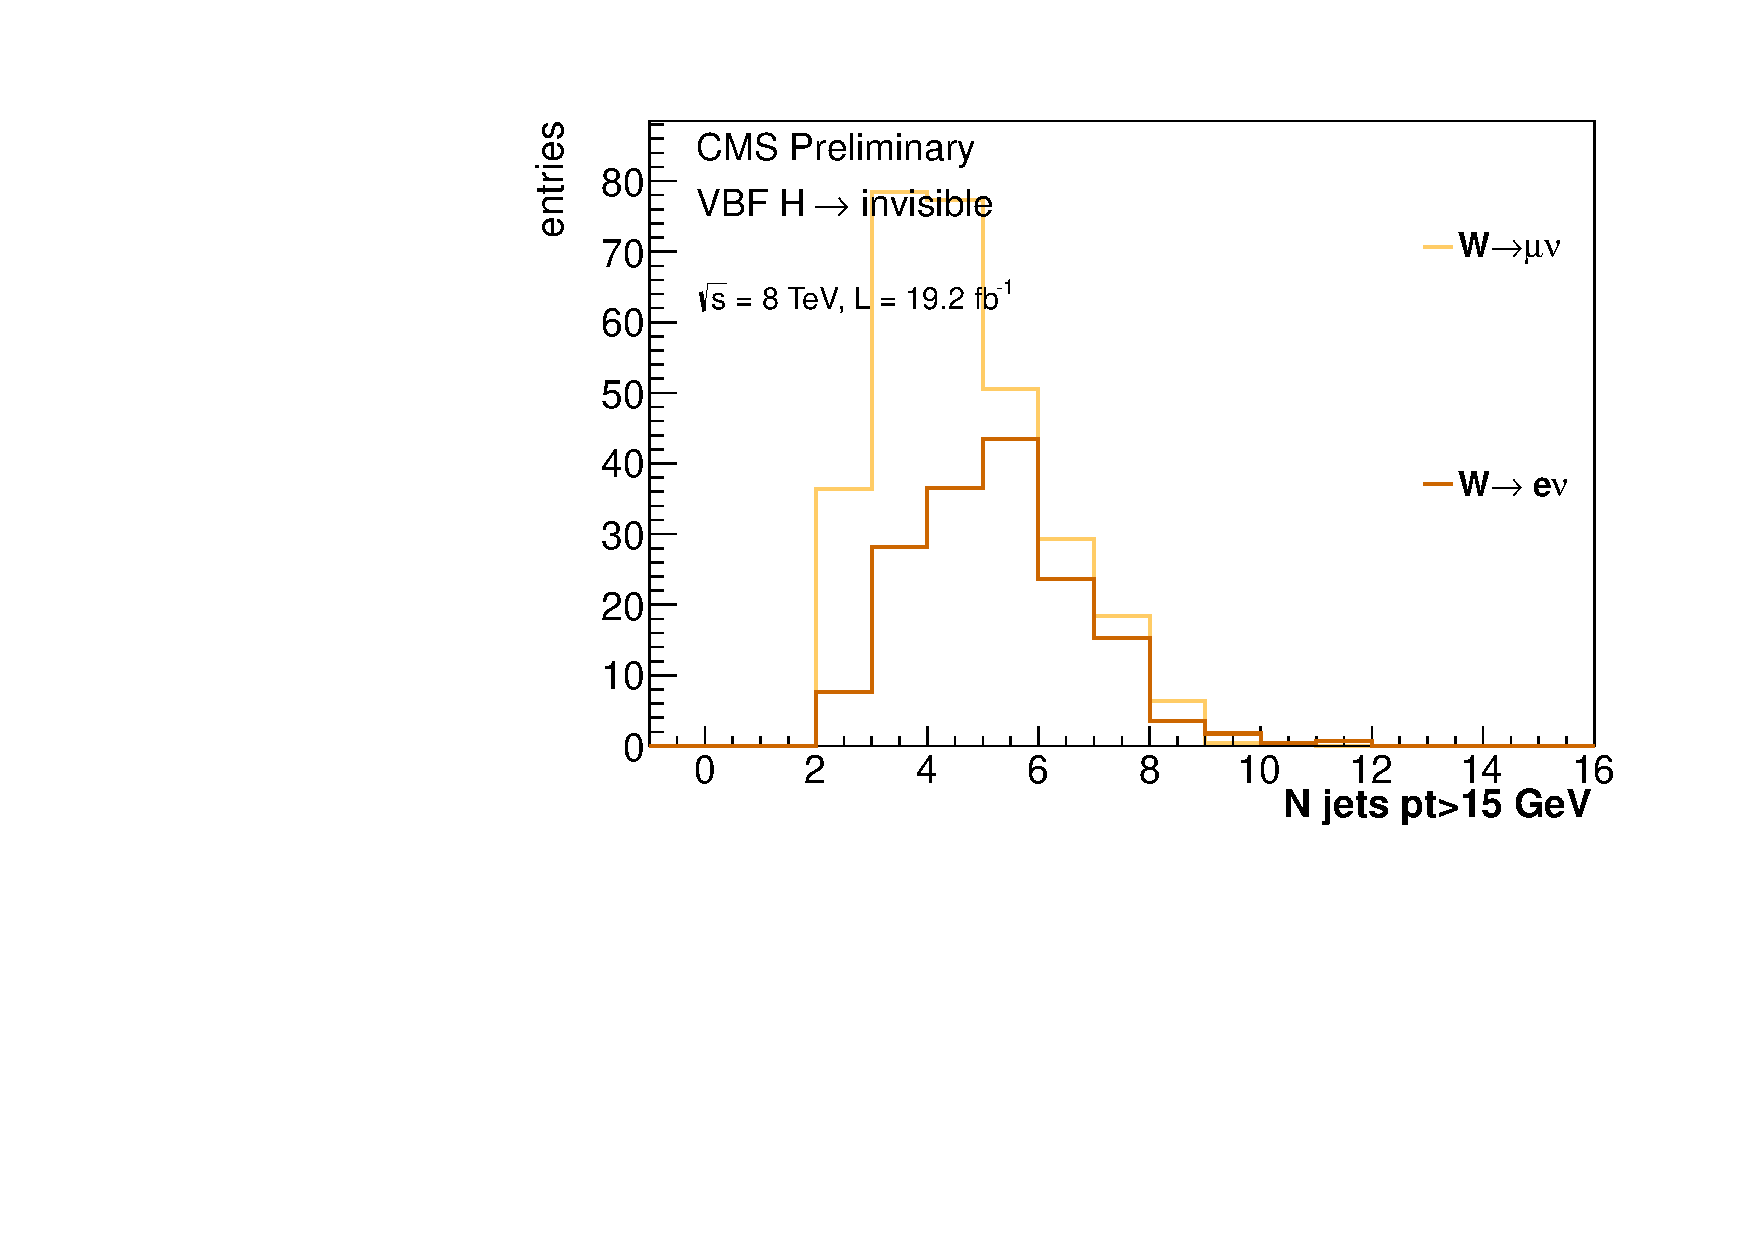
\includegraphics[width=.5\textwidth,clip=true,trim=0 0 0 30]{TalkPics/genlepstudy020315/outsideacceptance/nunu_n_jets_15.pdf}
    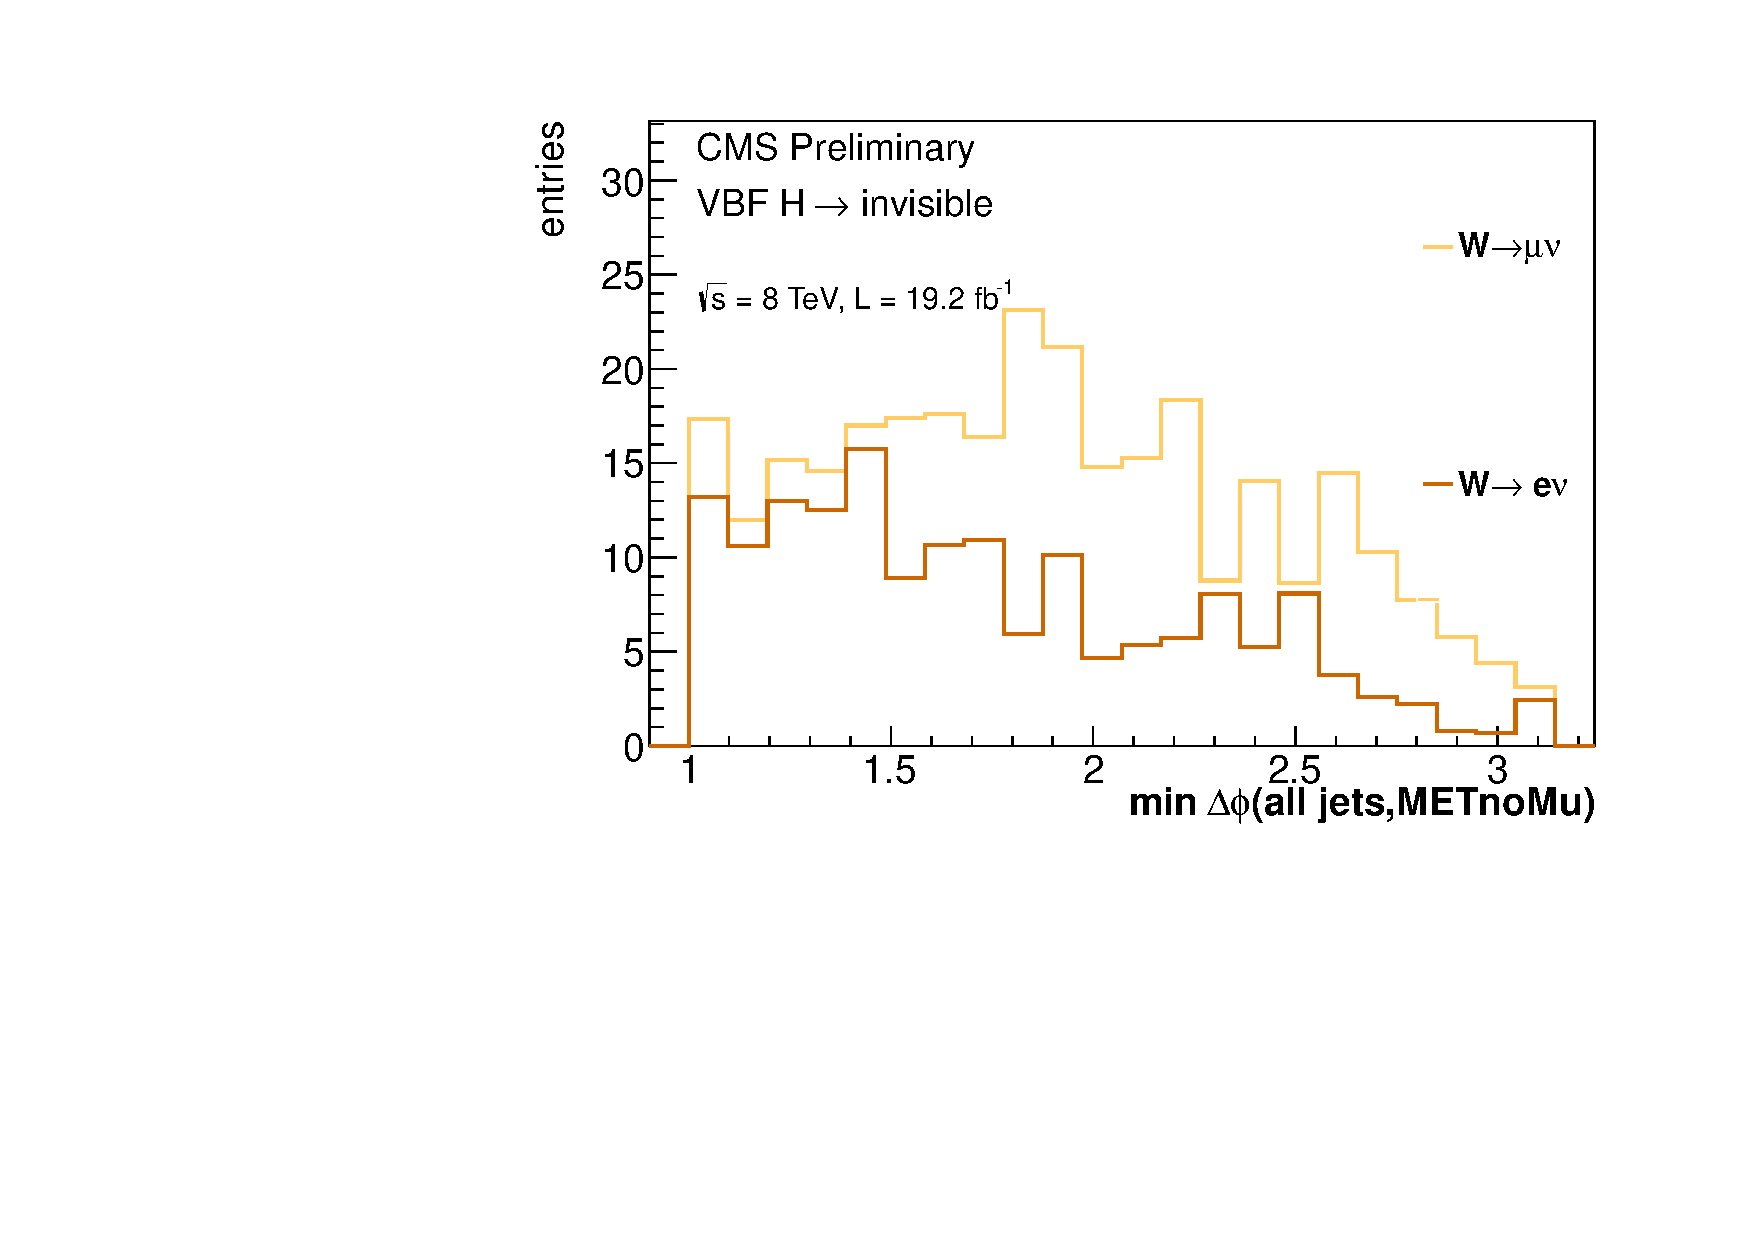
\includegraphics[width=.5\textwidth,clip=true,trim=0 0 0 30]{TalkPics/genlepstudy020315/outsideacceptance/nunu_alljetsmetnomu_mindphi.pdf}
  \end{center}
\end{frame}

\begin{frame}
  %!!SHOW NJETS, MINDPHI, GENLEPPT AS EVIDENCE FOR ELE BECOMING JETS OUTSIDE ACCEPTANCE
  \frametitle{Outside acceptance}
    \begin{block}{}
    \scriptsize
    \begin{itemize}
    \item Seems outside acceptance electrons are more likely to be reconstructed as jets than muons
    \item Loosen jetmetdphi cut to 1
    \end{itemize}
  \end{block}
  \begin{center}
    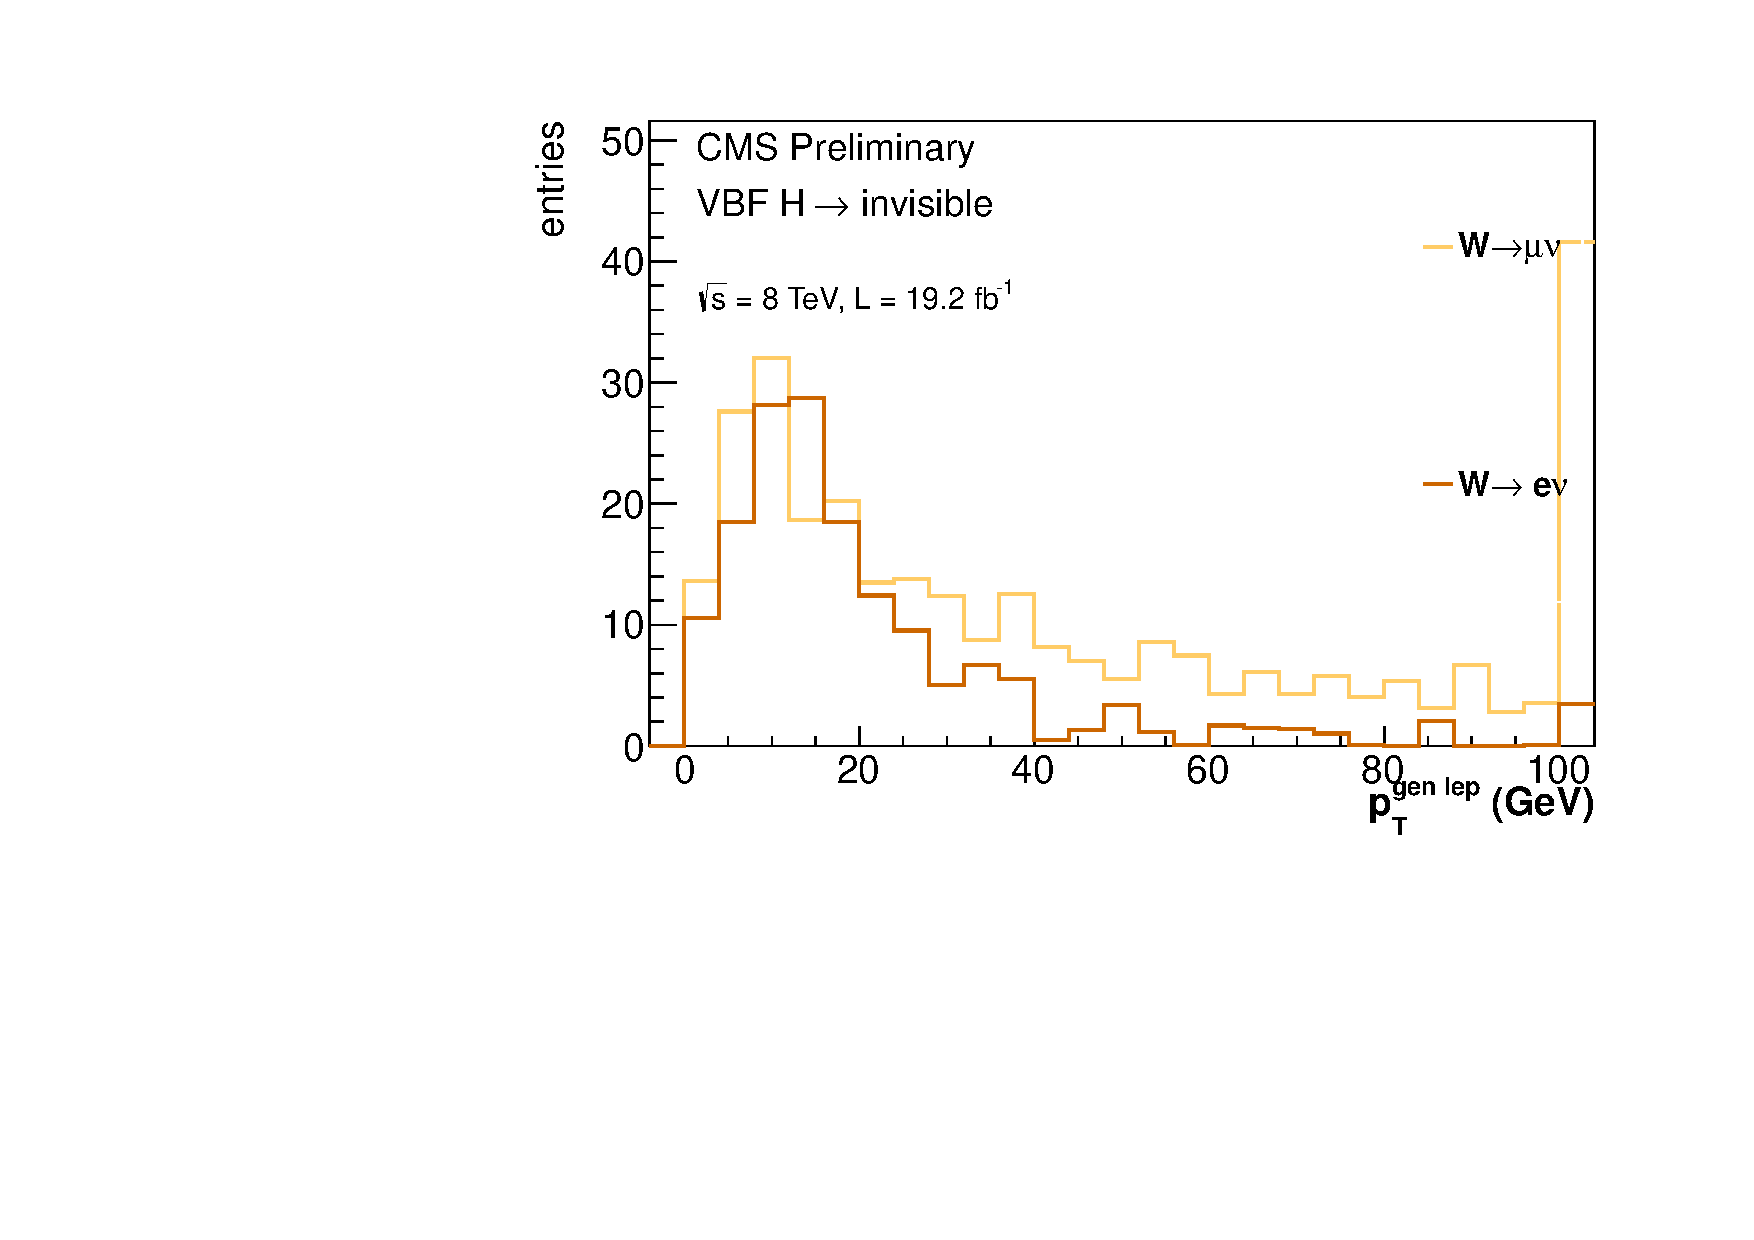
\includegraphics[width=.5\textwidth,clip=true,trim=0 0 0 30]{TalkPics/genlepstudy020315/outsideacceptance/nunu_genlep1_pt.pdf}
    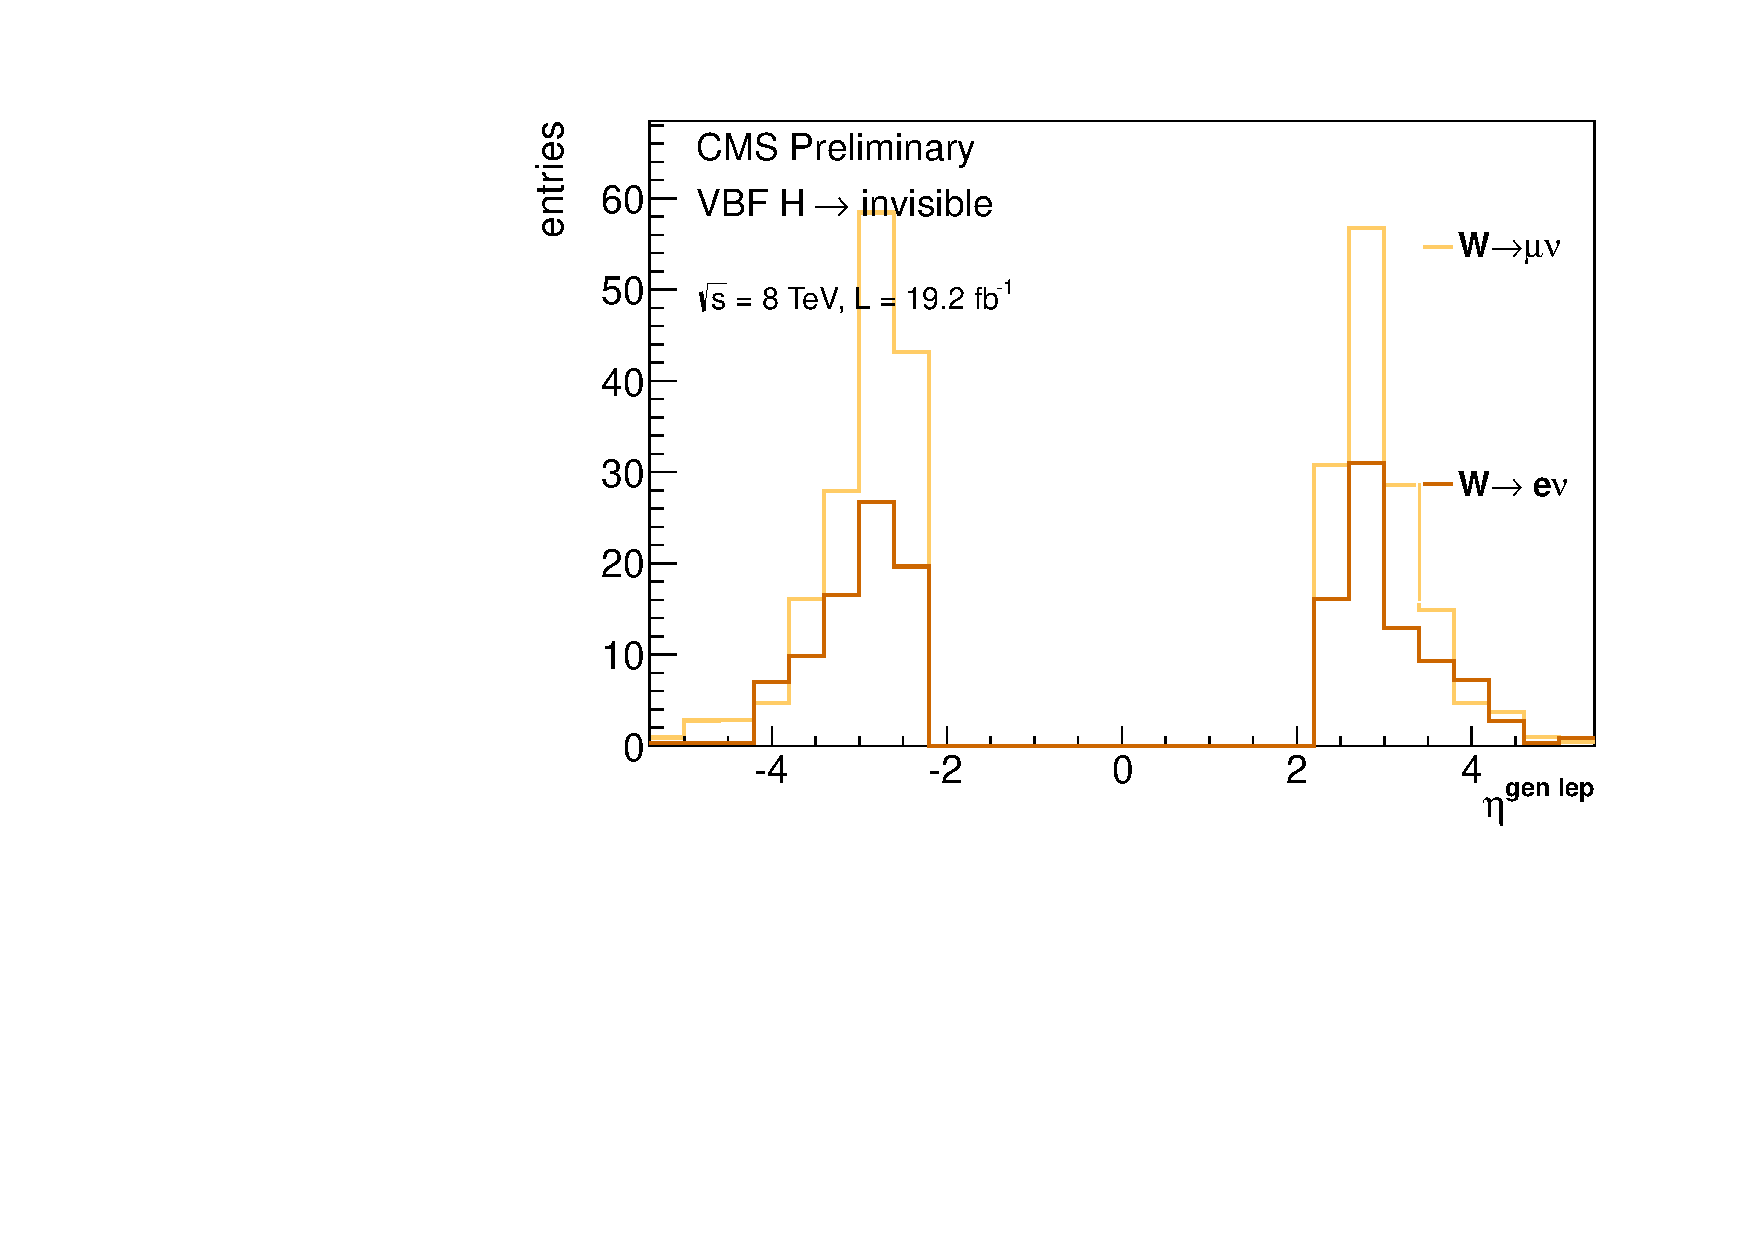
\includegraphics[width=.5\textwidth,clip=true,trim=0 0 0 30]{TalkPics/genlepstudy020315/outsideacceptance/nunu_genlep1_eta.pdf}
    \end{center}
\label{lastframe}
\end{frame}

\begin{frame}
  \frametitle{Backup}
\end{frame}

\end{fmffile}
\end{document}
